\chapter{Circular Waveguide (2)}\label{lec:lec45}
Before delving into the discussion of TE (Transverse Electric) modes in a circular waveguide, let us briefly revisit the TM (Transverse Magnetic) modes covered in the previous chapter. 

\section{TM modes in a circular waveguide}
Considering a circular waveguide filled with a dielectric material characterized by permeability $\mu$ and permittivity $\epsilon$, we recognize the presence of the $E_z$ component. The boundary condition for the conducting surface is fulfilled when $E_z(r=a) = 0$, indicating that the electric field component $E_z$ vanishes at the radial distance $r=a$. Upon solving for $E_z$ using equation~\eqref{eqn:electricfieldsoln}, we obtained the solution $E_z = A_n J_n(hr)\cos(n\phi)$, where $h = \omega^2\mu + \gamma^2$.

Upon further analysis, we have observed that certain modes satisfy the boundary condition, and these modes can be characterized by two parameters, namely $n$ and $p$. In this context, a specific TM mode is denoted as $TM_{np}$. The parameter $n$ not only represents the variation of the amplitude in $\phi$ but also corresponds to the order of the Bessel function involved in the solution. On the other hand, the parameter $p$ indicates the specific zero point (root) within the Bessel function, which enables the satisfaction of the boundary condition. Indeed, the modes in the circular waveguide are characterized by two aspects. Firstly, the variation of amplitude in the $\phi$ direction. It is represented by the term $\cos(n\phi)$ in the solution.

Secondly, the parameter $n$ determines the number of lobes or wavelengths in the azimuthal direction. Again, the parameter $n$ must be an integer. This is because the term $\cos(n\phi)$ must return to the same value after a complete cycle of $\phi=2\pi$. If the amplitude does not repeat itself after a full revolution, we do not have a mode. So the two values which define a mode are $n$ and $p$ where $n$ is the number of times we have variations in the azimuthal $\phi$, direction and based on the order of the Bessel function $p$, we determine which zero point (root) should be considered to satisfy the boundary condition which in the number of lobes we would get in the radial, $r$, direction.

From our study of the Bessel functions we recall that only $J_0(hr)$ has an amplitude at $hr = 0$ and the rest $J_n(hr)$ function has an amplitude which is zero at $hr = 0$ for $n \ne 0$. Also, we observed from the table that the lowest TM mode is the $TM_{01}$ mode where $n = 0$ and $p = 1$. $n = 0$ implies there is no variation in the $\phi$ direction and $p = 1$ shows that there is only one peak or lobe in the $r$ direction, therefore, $ha = 2.405$ from table~\ref{tab:rootsofbessel}. 

Now let us look at a colour 2D plot showing the electric field intensities for various TM modes.
\begin{figure}[h]
\centering
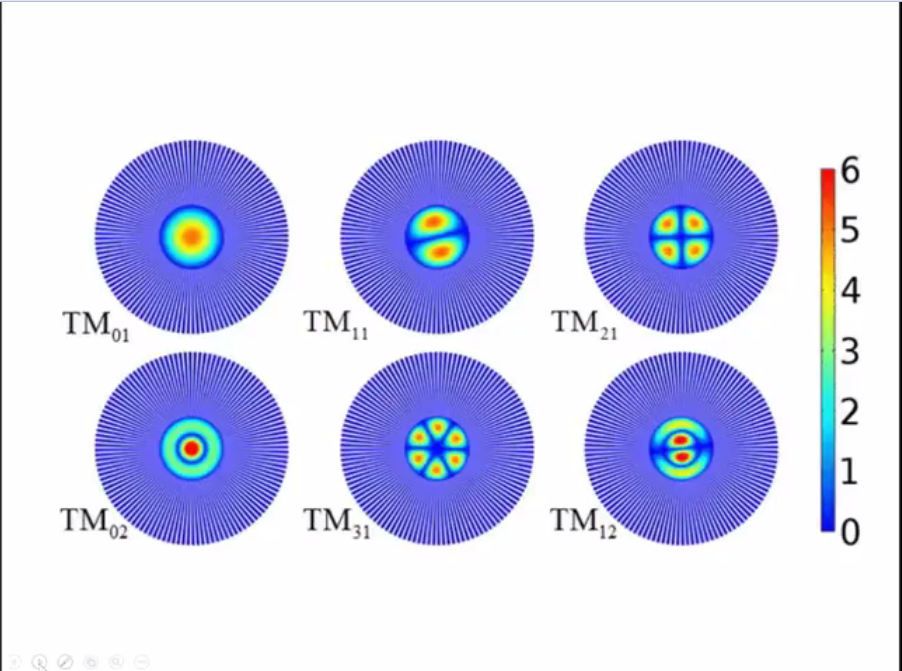
\includegraphics[width=0.9\linewidth]{\pathtoparttwo/graphics/colourplot}
\caption{2D colour plot of the TM modes.}
\label{fig:colourplot}
\end{figure}

\subsection{$TM_{10}$ mode}
In the $\phi$ direction, we observe that there is no variation since $n=0$. Also if we consider the $r$ direction, there is one lobe as shown in figure~\ref{fig:m1}.
\begin{figure}[h]
\centering
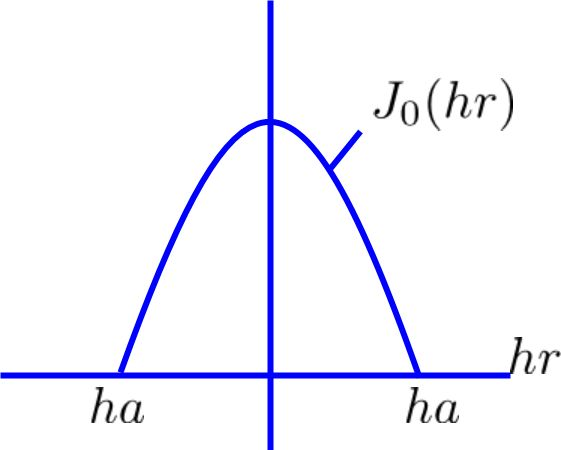
\includegraphics[width=0.5\linewidth]{\pathtoparttwo/graphics/m1}
\caption{Plot of Electric field variation in the $r$ direction for $TM_{10}$ mode.}
\label{fig:m1}
\end{figure}

We can observe from the plot that the field peaks at the centre and at zero at the boundary which is the same as the colour plot in figure~\ref{fig:colourplot}.
   
\subsection{$TM_{02}$ mode}
For the $TM_{02}$ mode, we observe that there is no variation in the azimuthal direction ($\phi$) since $n=0$. This implies that the field intensity remains constant along any circular path drawn in the waveguide.

In terms of the radial direction ($r$), we observe two peaks or lobes. However, it is important to note that these peaks have different magnitudes, which are represented by the red and cyan colours in the plot shown in figure~\ref{fig:colourplot}. 

To visualize the electric field variation for the $TM_{02}$ mode specifically in the radial direction, let us plot the graph accordingly.
\begin{figure}[h]
\centering
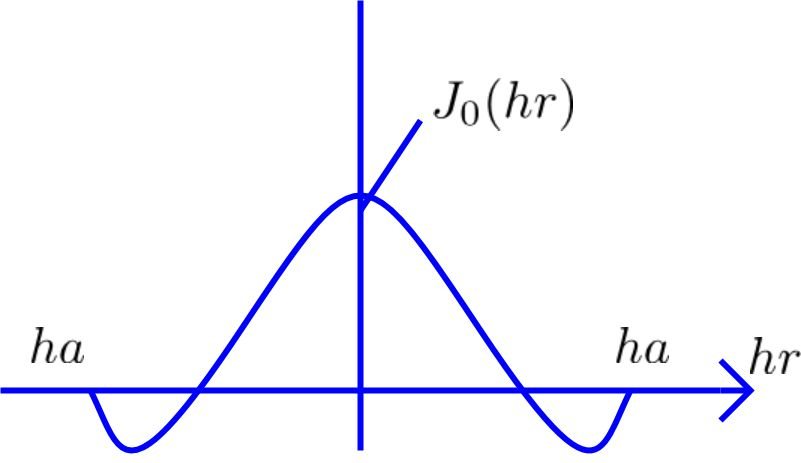
\includegraphics[width=0.7\linewidth]{\pathtoparttwo/graphics/m2}
\caption{Plot of the electric field variation in the $r$ direction for $TM_{02}$ mode.}
\label{fig:m2}
\end{figure}

The plot shown in figure~\ref{fig:m2} is consistent with the colour plot displayed in figure~\ref{fig:colourplot}. The magnitude at the centre of the circular waveguide corresponds to the red colour observed in the plot, while the cyan colour represents the negative lobes with lower amplitudes. This observation is in contrast to the behaviour observed in rectangular waveguides, where the amplitude of the electric field remains the same for all lobes.

To illustrate this difference further, let us consider the 3rd order mode in the y direction. The corresponding plot, as shown in figure~\ref{fig:m3}, demonstrates that the amplitude remains constant throughout the lobes. This is distinct from the behaviour observed in the circular waveguide, where the amplitude varies between the positive and negative lobes.

These distinctions highlight the unique characteristics of the electric field behaviour in different waveguide geometries.
\begin{figure}[h]
\centering
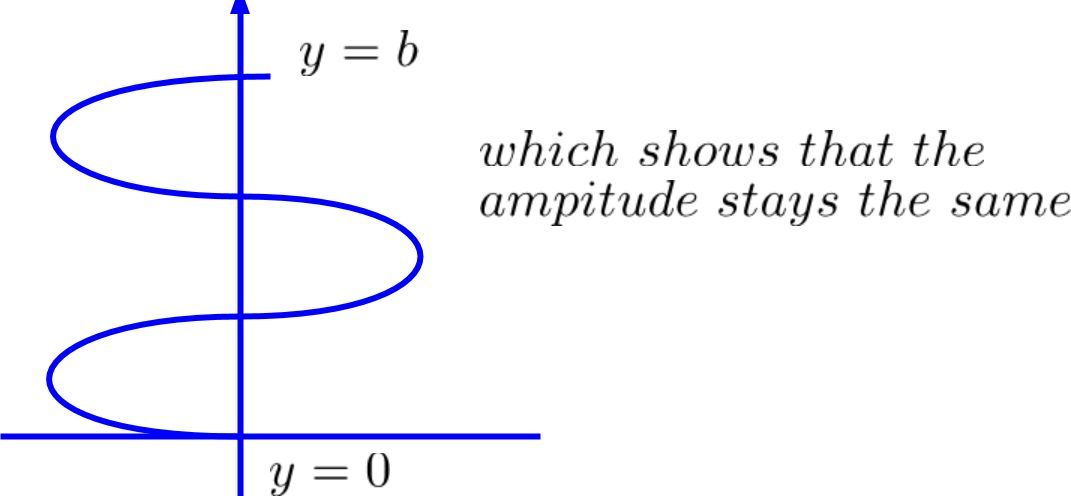
\includegraphics[width=0.5\linewidth]{\pathtoparttwo/graphics/m3}
\caption{Plot of the electric field variation in the $y$ direction for $TM_{x3}$ mode.}
\label{fig:m3}
\end{figure}

\subsection{$TM_{11}$ mode}
As depicted in figure~\ref{fig:colourplot}, we observe a single wavelength variation in the azimuthal direction ($\phi$). This is evident from the presence of two peaks, one representing the positive maximum and the other representing the negative minimum. The behaviour of these peaks aligns with the first-order Bessel function, specifically $J_1(hr)$.

In the case of this mode, $p=1$, indicating that the boundary condition is satisfied at the first root of $J_1(hr)$. It is important to recall that $J_1(hr)$ has a zero at $h_r=0$, which corresponds to the centre of the circular waveguide. Therefore, the deep blue colour observed in the plot signifies that there is no electric field at the centre of the waveguide.

\subsection{$TM_{21}$ mode}
The $TM_{21}$ mode is characterized by $n=2$, indicating that we expect two wavelengths in the azimuthal direction ($\phi$). This corresponds to the presence of four peaks: two maximums and two minimums, as depicted in figure~\ref{fig:colourplot}.

Considering $p=1$ for this mode, we anticipate a single peak in the radial direction ($r$). The plot shown in figure~\ref{fig:m4} illustrates the variation of the electric field in the $r$ direction for the $TM_{21}$ mode.
\begin{figure}[h]
\centering
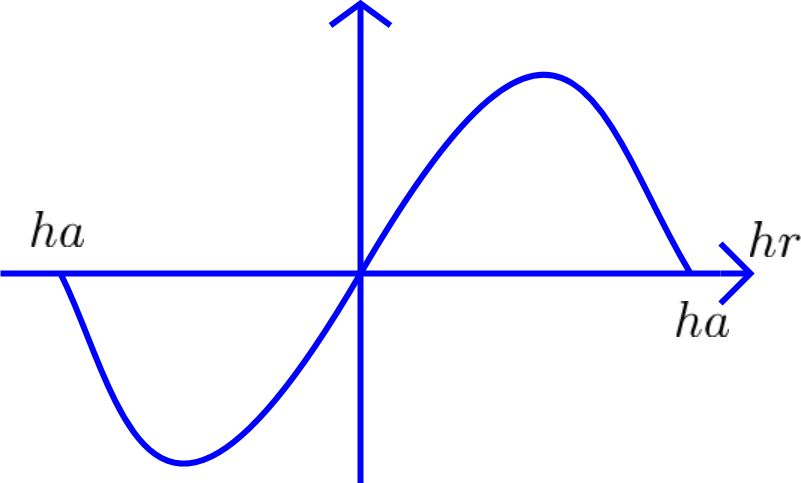
\includegraphics[width=0.5\linewidth]{\pathtoparttwo/graphics/m4}
\caption{Plot of the electric field variations for $TM_{21}$ mode.}
\label{fig:m4}
\end{figure}

\subsection{$TM_{31}$ mode}
The $TM_{31}$ mode corresponds to $n=3$, indicating three wavelengths in the azimuthal direction ($\phi$). As a result, we observe six peaks or lobes in this direction. Each peak represents a maximum or minimum point of the electric field.

Additionally, considering $p=1$ for this mode means that we apply the boundary condition at the first zero point of the Bessel function. This choice ensures that the electric field satisfies the boundary condition at a specific radial position in the waveguide.

\subsection{$TM_{12}$ mode}
In the case of the $TM_{12}$ mode, we have $n=1$, which corresponds to one wavelength in the azimuthal direction ($\phi$). This results in two lobes or peaks in the $\phi$ direction.

For $p=2$, we consider the second root of the $J_1(hr)$ function. This implies that we expect two lobes in the radial direction ($r$). The colour plot in figure~\ref{fig:colourplot} for the $TM_{12}$ mode showcases this behaviour, with two distinct lobes in the radial direction.

In summary, the parameter $n$ represents the number of wavelengths in the azimuthal direction ($\phi$), while $p$ denotes the number of lobes in the radial direction ($r$).
   
\section{TE modes in a circular waveguide}
Now, let's take a look at the TE modes of the circular waveguide. For this mode, we need to study the derivative of the Bessel function. From equation~\eqref{eqn:besselsolnseries2}, we can see that the Bessel function is given as 
\begin{align*}
J_n(x) &= \sum_{k = 0}^{\infty}\frac{(-1)^k (\frac{x}{2})^{2k + n}}{k! \Gamma(n + k + 1)}\quad\text{But, }\Gamma(n + k + 1) = (n+k)!\\
&= \sum_{k = 0}^{\infty}\frac{(-1)^k (\frac{x}{2})^{2k + n}}{k! (n + k)!}\quad\text{Substituting }x = hr\\
J_n(hr) &= \sum_{k = 0}^{\infty}\dfrac{(-1)^k(hr)^{2k + n}}{k!(k+n)!2^{2k + n}} \quad \text{where n is an interger}
\end{align*}
So the derivative of the Bessel function is given as $ \derivative{J_n(hr)}{r} $ and it is denoted by $J'_n(hr) $ and it is given as 
\begin{align*}
J'_n(hr) &= \sum_{k = 0}^{\infty}\dfrac{(-1)^k h^{2k + n}(2k + n)r^{2k + n -1}}{k!(k+n)!2^{2k + n}}\\
&= \frac{1}{2}\bigg[J_{n-1}(hr) - J_{n + 1}(hr)\bigg]\footnotemark
\end{align*}
\footnotetext{
By differentiating $J_n(hr)$ with respect to $r$ and further simplifying the expression, we obtain the above relationship.
}
Indeed, for the circular waveguide, the application of the boundary condition leads us to consider specific numerical values of $hr$ at which the derivative of the Bessel function, $J'_n(hr)$, equals zero. These values of $hr$ are essential for determining the characteristics and properties of the waveguide modes.

However, it is important to note that this relationship and the zeros of the derivative of the Bessel function are particularly useful when dealing with dielectric waveguides, such as optical fibres. In the context of the circular waveguide, we primarily focus on the numerical values that satisfy the boundary condition rather than explicitly utilizing the relationship mentioned.

For further reference and analysis, Table~\ref{tab:zerosofdiffbessel} provides the specific values of $hr$ where $J'_n(hr)$ vanishes, which are crucial for solving the modes of the circular waveguide.
\begin{table}[h]
\centering
\text{Zeros of $J'_n(hr)$}\\
\begin{tabular}{|c | c c c|}
\hline
\backslashbox{p}{n} & n=0 & n=1 & n=2 \\
\hline
1 & 3.832 & 1.841 & 3.054 \\
2 & 7.016 & 5.331 &6.706 \\
\hline
\end{tabular}
\label{tab:zerosofdiffbessel}
\end{table}

From the table, we observe that the lowest zero point is when $n = 1$ and $p = 1$ and this corresponds to a $TE_{11}$ mode therefore the $TE_{11}$ mode is the lowest cut-off mode, followed by $TE_{21}$ and then $TE_{01}$ and so on.

For the TE mode we know that $E_z = 0$ and $H_z$ exists, so we will solve for the $H_z$  component which is given as;
\begin{align*}
H_z(r,\phi,z) = H_z(r,\phi)e^{-\gamma z}
\end{align*}
So, the Helmholtz equation becomes
\begin{equation}
\nabla^2 H_z(r,\phi) + h^2 H_z(r,\phi) = 0
\label{eqn:helmholtztemode}
\end{equation}
To solve this equation we repeat the procedure we carried out for the TM mode such that 
\begin{align*}
H_z(r,\phi)= R(r)\Phi(\phi)
\end{align*}
Therefore equation~\eqref{eqn:helmholtztemode} becomes
\begin{align*}
\frac{1}{r}\partialderivative{}{r}\bigg(r\partialderivative{R\Phi}{r}\bigg) + \frac{1}{r^2}\partialderivative[2]{R\Phi}{\phi} + h^2\{R\Phi\} = 0
\end{align*}
Thus, the two solutions are given as
\begin{equation}
\derivative[2]{R}{r} + \frac{1}{r^2}\derivative{R}{r} + \bigg(h^2 - \frac{n^2}{r^2}\bigg)R = 0
\label{eqn:radialtemode}
\end{equation}
and 
\begin{equation}
\dfrac{d^2\Phi}{d\phi^2} + n^2\Phi = 0
\label{eqn:angulartemode}
\end{equation}
The procedure is similar to that of the TM mode, the only difference is that we start with solving the Helmholtz wave equation for the magnetic field. So the solution of the magnetic field is 
\begin{align*}
H_z(r,\phi) = A_nJ_n(hr)\cos(n\phi)\quad\text{n has to be an integer}
\end{align*}
We can now solve for the other components. From equations~\eqref{eqn:transverseele2} and~\eqref{eqn:transversemag2} we have
\begin{align*}
\bar{E}_\perp = \frac{-j\omega\mu}{h^2}\nabla_\perp\times(H_z\hat{z}) - \frac{\gamma}{h^2}\nabla_\perp E_z\\
\bar{H}_\perp = \frac{j\omega\epsilon}{h^2}\nabla_\perp\times(E_z\hat{z}) - \frac{\gamma}{h^2}\nabla_\perp H_z
\end{align*}

For the TE mode, $E_z = 0$, therefore,
\begin{dmath} 
\bar{H}_\perp = H_r \hat{r} + H_\phi \hat{\phi} = \frac{-\gamma}{h^2}\nabla_\perp H_z
= \frac{-\gamma}{h^2}\bigg\{ 
\hat{r}\partialderivative{H_z}{r} + \frac{\hat{\phi}}{r}\partialderivative{H_z}{\phi}  
\bigg\}
\end{dmath}
Therefore
\begin{align*}
H_r = \frac{-\gamma}{h^2}\partialderivative{H_z}{r} = \frac{-\gamma}{h^2}A_nJ'_n(hr)\cos(n\phi)
\end{align*}
For a lossless medium $ \gamma =j\beta$, so 
\begin{align*}
H_r = \frac{-j\beta}{h^2}A_nJ'_n(hr)\cos(n\phi)
\end{align*}
Similarly, for the $\phi$ component, we have
\begin{align*}
H_\phi = \frac{-j\beta}{h^2}\frac{\partial H_z}{\partial \phi} = \frac{-j\beta n}{h^2 r}A_nJ'_n(hr)\sin(n\phi)
\end{align*}

For the transverse electric field, we have
\begin{dmath} 
\bar{E}_\perp = \frac{-j\omega\mu}{h^2}\nabla_\perp\times H_z\hat{z}
=\frac{-j\omega\mu}{h^2}
\left\{ 
\frac{1}{r}
\begin{vmatrix}
\hat{r} & r\hat{\phi} & \hat{z}\\ 
\partialderivative{}{r} & \partialderivative{}{\phi} & 0\\
0 & 0 & H_z
\end{vmatrix}
\right\}
= E_r\hat{r} + E_\phi\hat{\phi}
= \frac{j\omega\mu}{h^2} \bigg\{\frac{1}{r}\partialderivative{H_z}{\phi} - \partialderivative{H_z}{r}\bigg\}
\end{dmath}
Therefore, the components are
\begin{align*}
E_r &= \frac{-j\omega\mu}{h^2 r}\partialderivative{H_z}{\phi} = \frac{j\omega\mu n}{h^2 r}A_nJ_n(hr)\sin(n\phi)\\
E_\phi &= \frac{j\omega\mu}{h^2 }\partialderivative{H_z}{\phi} = \frac{j\omega\mu }{h^2 }A_nJ'_n(hr)\cos(n\phi)
\end{align*}
So the component is
\begin{align}
H_r &= \frac{j\beta}{h^2 }A_nJ_n(hr)\cos(n\phi)\\ H_\phi &= \frac{j\beta}{h^2 r}A_nJ_n(hr)\sin(n\phi)\\
H_z &= A_nJ_n(hr)\cos(n\phi)\\
E_r &= \frac{j\omega\mu n}{h^2 r}A_nJ_n(hr)\sin(n\phi)\\
E_\phi &= \frac{j\omega\mu }{h^2 }A_nJ_n(hr)\cos(n\phi)\\
E_z & = 0
\end{align}

In the context of the circular waveguide, we have observed that the transverse components of the magnetic field, namely $H_r$ and $H_\phi$, are directly related to the derivative of the field component in the longitudinal direction, $H_z$. Specifically, $H_r$ is proportional to $\partialderivative{H_z}{r}$, while $H_\phi$ is proportional to $\partialderivative{H_z}{\phi}$.

Similarly, the transverse components of the electric field, $E_r$ and $E_\phi$, are related to the derivative of the field component in the longitudinal direction, $H_z$. In this case, $E_r$ is proportional to $\partialderivative{H_z}{\phi}$, and $E_\phi$ is proportional to $\partialderivative{H_z}{r}$.

For the TE (Transverse Electric) mode, we specifically observed that the electric field component $E_\phi$ is parallel to the conducting walls of the waveguide. This is illustrated in Figure~\ref{fig:m5}, where the electric field lines are tangential to the walls of the circular waveguide.
\begin{figure}[h]
\centering
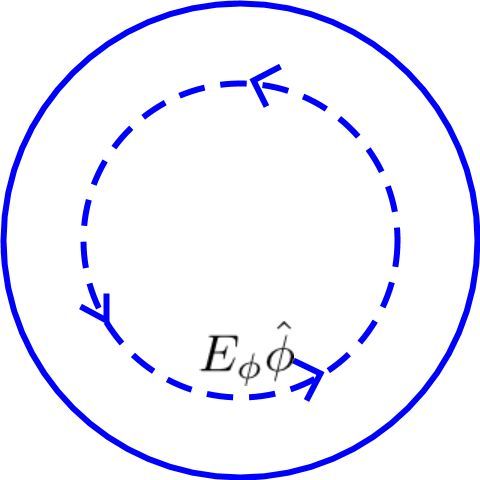
\includegraphics[width=0.5\linewidth]{\pathtoparttwo/graphics/m5}
\caption{Azimuthal electric field component for the TE mode}
\label{fig:m5}
\end{figure}

Again, the electric field component $E_\phi$ must go to zero at the boundary ($r=0$) to satisfy the boundary condition. This requirement leads to the condition $J'_n(ha) = 0$, where $ha$ represents the product of the waveguide radius $a$ and the radial component $h$ of the waveguide mode.

By referring to Table~\ref{tab:zerosofdiffbessel}, we can observe that the smallest value of $ha$ for which the boundary condition is satisfied is $ha = 1.841$. This corresponds to the TE mode with the lowest cut-off frequency. In this mode, we have one wavelength variation in the azimuthal direction ($\phi$) due to $n=1$, and $p=1$ indicates that we are considering the first zero point of the derivative of the Bessel function, specifically $J'_1(hr)$.

So
$$
(h)_{TE_{11}} = \frac{1.841}{a}
$$
And the cut-off frequency of this mode is 
$$
(f_c)_{TE_{11}} = \frac{(h)_{TE_{11}}}{2\pi\sqrt{\mu\epsilon}} = \frac{0.293}{a\sqrt{\mu\epsilon}}
$$
We recall that the lowest TE mode is the $TE_{01}$ mode which corresponds to $(f_c)_{TE_{01}} = \frac{0.383}{a\sqrt{\mu\epsilon}}$. It is worth noting that the cut-off frequency of the $TE_{11}$ mode is lower than that of the $TE_{01}$ mode.

As a result, the $TE_{11}$ mode becomes the dominant mode in the circular waveguide. The modes in the circular waveguide are not arranged in a simple order like in the rectangular waveguide due to the presence of the derivative of the Bessel function in the boundary condition. However, by referring to the table, we can observe that the modes are ordered based on their cut-off frequencies, from lowest to highest, as $TE_{11}, TE_{21}, TE_{01}, TE_{12}, TE_{22}$, and $TE_{02}$.

\section{Attenuation in the circular waveguide}
In terms of losses, the behaviour in the circular waveguide is similar to that of the parallel plane waveguide. The modes that have more energy close to the conducting wall will experience more losses because this energy can excite currents on the conducting surfaces. 

For the TE (Transverse Electric) mode, which includes both the $H_z$ and $H_\phi$ components, and the TM (Transverse Magnetic) mode, which includes the $H_\phi$ component, the losses generally decrease as the frequency increases and then start to increase. This is a common trend. 

However, there are unique modes of the order $TE_{0p}$. In such modes, the losses decrease monotonically as the frequency increases. This is demonstrated in figure~\ref{fig:m6} for the specific case of the $TE_{01}$ mode.

It is important to note that the specific loss behaviour in different modes and frequency ranges can vary, but the general trend described above provides an understanding of the behaviour of losses in the circular waveguide.
\begin{figure}[h]
\centering
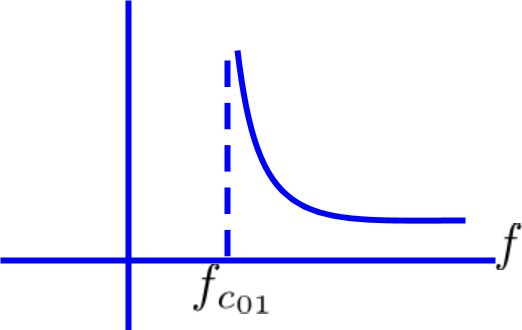
\includegraphics[width=.5\linewidth]{\pathtoparttwo/graphics/m6}
\caption{Attenuation in the $TE_{01}$ mode}
\label{fig:m6}
\end{figure}

Indeed, the $TE_{0p}$ mode in the circular waveguide exhibits a unique behaviour where the losses decrease monotonically as the frequency increases. This behaviour is distinct and not observed in any other mode, whether in a circular or rectangular waveguide. Therefore, the $TE_{0p}$ mode stands out in terms of its loss characteristics. This concludes our discussion on the circular waveguide.
